\section{Experiments}
\label{sec:results}

In this section we describe the results of many experiments, comparing our Matching Networks model against strong baselines.
All of our experiments revolve around the same basic task: an $N$-way $k$-shot learning task.
Each method is providing with a set of $k$ labelled examples from each of $N$ classes that have not previously been trained upon.
The task is then to classify a disjoint batch of unlabelled examples into one of these $N$ classes.
Thus random performance on this task stands at $1/N$.
We compared a number of alternative models, as baselines, to Matching Networks.

Let $L'$ denote the held-out subset of labels which we only use for one-shot. Unless otherwise specified, training is always on $\neq\!\! L'$, and test in one-shot mode on $L'$.

We ran one-shot experiments on three data sets: two image classification sets (Omniglot \cite{omniglot} and ImageNet \cite[ILSVRC-2012]{ImageNet}) and one language modeling (Penn Treebank).
The experiments on the three data sets comprise a diverse set of qualities in terms of complexity, sizes, and modalities. 

\subsection{Image Classification Results}

\begin{table}[b]\small
\begin{center}
\begin{tabular}{l@{\hskip \colspaceL}l@{\hskip \colspaceL}l@{\hskip \colspaceL}r@{\hskip \colspaceS}r@{\hskip \colspaceL}r@{\hskip \colspaceS}r@{\hskip \colspaceS}r}
\toprule
\multirow{2}{*}{\b{Model}} & \multirow{2}{*}{\b{Matching Fn}} & \multirow{2}{*}{\b{Fine Tune}} & \multicolumn{2}{c}{\b{5-way Acc}} &  \multicolumn{2}{c}{\b{20-way Acc}}\\
~ &  ~ & ~ &1-shot & 5-shot & 1-shot & 5-shot \\
\midrule
\b{\abbr{Pixels}} & Cosine & N & \t{41.7\%} & \t{63.2\%} & \t{26.7\%} & \t{42.6\%} \\
\b{\abbr{Baseline Classifier}} & Cosine & N & \t{80.0\%} & \t{95.0\%} & \t{69.5\%} & \t{89.1\%} \\
\b{\abbr{Baseline Classifier}} & Cosine & Y & \t{82.3\%} & \t{98.4\%} & \t{70.6\%} & \t{92.0\%} \\
\b{\abbr{Baseline Classifier}} & Softmax & Y & \t{86.0\%} & \t{97.6\%} & \t{72.9\%} & \t{92.3\%} \\
\midrule
\b{\abbr{MANN (No Conv) \cite{mann}}} & Cosine & N & \t{82.8\%} & \t{94.9\%} & \t{~--} & \t{~--} \\
\b{\abbr{Convolutional Siamese Net \cite{siamese}}} & Cosine & N & \t{96.7\%} & \t{98.4\%} & \t{88.0\%} & \t{96.5\%} \\
\b{\abbr{Convolutional Siamese Net \cite{siamese}}} & Cosine & Y & \t{97.3\%} & \t{98.4\%} & \t{88.1\%} & \t{97.0\%} \\
\midrule
\b{\abbr{Matching Nets (Ours)}} & Cosine & N & \b{98.1\%} & \b{98.9\%} & \b{93.8\%} & \t{98.5\%} \\
\b{\abbr{Matching Nets (Ours)}} & Cosine & Y & \t{97.9\%} & \t{98.7\%} & \t{93.5\%} & \b{98.7\%} \\
\bottomrule
\end{tabular}
\end{center}
\caption{
\label{tab:omniglot}
Results on the Omniglot dataset.
}
\end{table}

For vision problems, we considered four kinds of baselines: matching on raw pixels, matching on discriminative features from a state-of-the-art classifier (Baseline Classifier), MANN \cite{mann}, and our reimplementation of the Convolutional Siamese Net \cite{siamese}.
The baseline classifier was trained to classify an image into one of the original classes present in the training data set, but excluding the $N$ classes so as not to give it an unfair advantage (i.e., trained to classify classes in $\neq\!\! L'$).
We then took this network and used the features from the last layer (before the softmax) for nearest neighbour matching, a strategy commonly used in computer vision \cite{donahue2014decaf} which has achieved excellent results across many tasks.
Following \cite{siamese}, the convolutional siamese nets were trained on a same-or-different task of the original training data set and then the last layer was used for nearest neighbour matching.

We also tried further fine tuning the features using only the support set $S'$ sampled from $L'$. This yields massive overfitting, but given that our networks are highly regularized, can yield extra gains. Note that, even when fine tuning, the setup is still one-shot, as only a single example per class from $L'$ is used.

\subsubsection{Omniglot}

Omniglot \cite{omniglot} consists of 1623 characters from 50 different alphabets.
Each of these was hand drawn by 20 different people.
The large number of classes (characters) with relatively few data per class (20),
makes this an ideal data set for testing small-scale one-shot classification.
The $N$-way Omniglot task setup is as follows: pick $N$ unseen character classes, independent of alphabet, as $L$.
Provide the model with one drawing of each of the $N$ characters as $S \sim L$ and a batch $B \sim L$.
Following \cite{mann},  we augmented the data set with random rotations by multiples of 90 degrees and used 1200 characters for training, and the remaining character classes for evaluation.

We used a simple yet powerful CNN as the embedding function -- consisting of a stack of modules, each of which is a $3\times 3$ convolution with 64 filters followed by batch normalization \cite{ioffe2015batch}, a Relu non-linearity and $2\times 2$ max-pooling. We resized all the images to $28\times 28$ so that, when we stack 4 modules, the resulting feature map is $1\times 1\times 64$, resulting in our embedding function $f(x)$. A fully connected layer followed by a softmax non-linearity is used to define the Baseline Classifier.

Results comparing the baselines to our model on Omniglot are shown in Table~\ref{tab:omniglot}.
For both $1$-shot and $5$-shot, $5$-way and $20$-way, our model outperforms the baselines. There are no major surprises in these results: using more examples for k-shot classification helps all models, and 5-way is easier than 20-way. We note that the Baseline Classifier improves a bit when fine tuning on $S'$, and using cosine distance versus training a small softmax from the small training set (thus requiring fine tuning) also performs well. Siamese nets fare well versus our Matching Nets when using 5 examples per class, but their performance degrades rapidly in one-shot. Fully Conditional Embeddings (FCE) did not seem to help much and were left out of the table due to space constraints.

Like the authors in \cite{siamese}, we also test our method trained on Omniglot on a completely disjoint task -- one-shot, 10 way MNIST classification. The Baseline Classifier does about 63\% accuracy whereas (as reported in their paper) the Siamese Nets do 70\%. Our model achieves 72\%.

\subsubsection{ImageNet}
\label{sec:imagenet}

Our experiments followed the same setup as Omniglot for testing, but we considered a \emph{rand} and a \emph{dogs} (harder) setup. In the \emph{rand} setup, we removed 118 labels at random from the training set, then tested only on these 118 classes (which we denote as $L_{rand}$). For the \emph{dogs} setup, we removed all classes in ImageNet descended from dogs (totalling 118) and trained on all non-dog classes, then tested on dog classes ($L_{dogs}$).
ImageNet is a notoriously large data set which can be quite a feat of engineering and infrastructure to run experiments upon it, requiring many resources.
Thus, as well as using the full ImageNet data set, we devised a new data set -- \emph{mini}ImageNet -- consisting of $60,000$ colour images of size $84\times 84$ with $100$ classes, each having $600$ examples. This dataset is more complex than CIFAR10 \cite{krizhevsky2010convolutional}, but fits in memory on modern machines, making it very convenient for rapid prototyping and experimentation. This dataset is fully described in Appendix~\ref{mi_desc}.
We used $80$ classes for training and tested on the remaining $20$ classes.
In total, thus, we have \emph{rand}ImageNet, \emph{dogs}ImageNet, and \emph{mini}ImageNet.

The results of the \emph{mini}ImageNet experiments are shown in Table~\ref{tab:miniim}. As with Omniglot, Matching Networks outperform the baselines.
However, \emph{mini}ImageNet is a much harder task than Omniglot which allowed us to evaluate Full Contextual Embeddings (FCE) sensibly (on Omniglot it made no difference).
As we an see, FCE improves the performance of Matching Networks, with and without fine tuning, typically improving performance by around two percentage points. 

\begin{figure}[t]
\centering
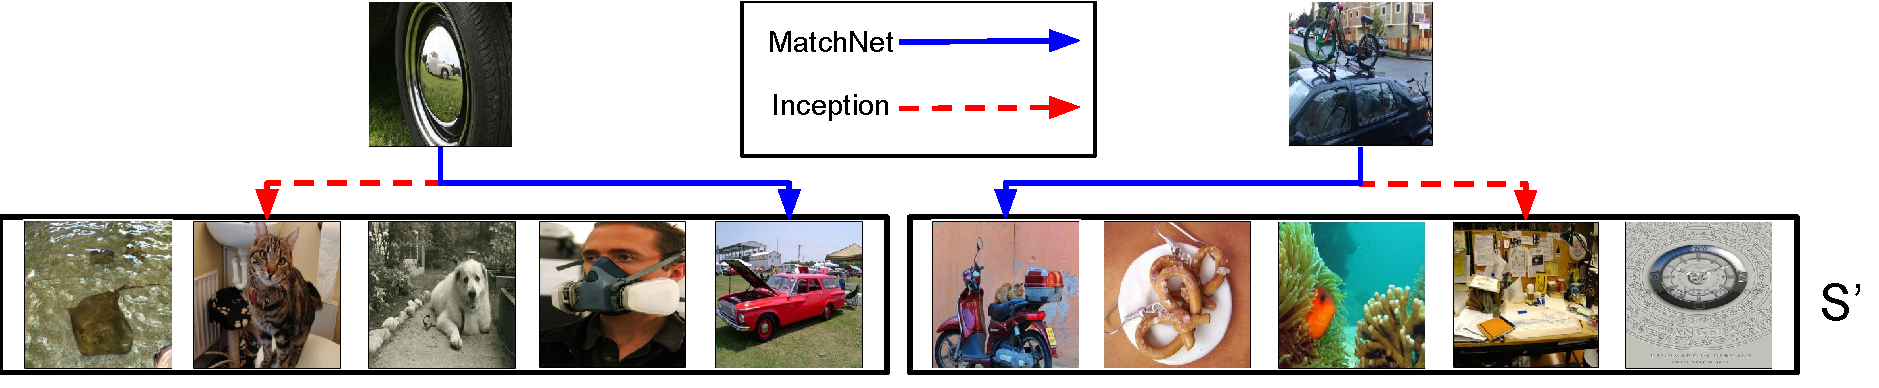
\includegraphics[width=1.0\textwidth]{figure_images}
\caption{\label{fig:imgs}Example of two 5-way problem instance on ImageNet. The images in the set $S'$ contain classes never seen during training. Our model makes far less mistakes than the Inception baseline. }
\end{figure}

\begin{table}[t]\small
\caption{
\label{tab:miniim}
Results on \emph{mini}ImageNet.
}
\begin{center}
\begin{tabular}{l@{\hskip \colspaceL}l@{\hskip \colspaceL}l@{\hskip \colspaceL}r@{\hskip \colspaceS}r@{\hskip \colspaceL}}
\toprule
\multirow{2}{*}{\b{Model}} & \multirow{2}{*}{\b{Matching Fn}} & \multirow{2}{*}{\b{Fine Tune}} & \multicolumn{2}{c}{\b{5-way Acc}} \\
~ &  ~ & ~ &1-shot & 5-shot \\
\midrule
\b{\abbr{Pixels}} & Cosine & N & \t{23.0\%} & \t{26.6\%} \\
\b{\abbr{Baseline Classifier}} & Cosine & N & \t{36.6\%} & \t{46.0\%} \\
\b{\abbr{Baseline Classifier}} & Cosine & Y & \t{36.2\%} & \t{52.2\%} \\
\b{\abbr{Baseline Classifier}} & Softmax & Y & \t{38.4\%} & \t{51.2\%} \\
\midrule
\b{\abbr{Matching Nets (Ours)}} & Cosine & N & \t{41.2\%} & \t{56.2\%} \\
\b{\abbr{Matching Nets (Ours)}} & Cosine & Y & \t{42.4\%} & \t{58.0\%} \\
\b{\abbr{Matching Nets (Ours)}} & Cosine (FCE) & N & \t{44.2\%} & \t{57.0\%} \\
\b{\abbr{Matching Nets (Ours)}} & Cosine (FCE) & Y & \b{46.6\%} & \b{60.0\%} \\
\bottomrule
\end{tabular}
\end{center}
\end{table}

Next we turned to experiments based upon full size, full scale ImageNet.
Our baseline classifier for this data set was Inception \cite{szegedy2015rethinking} trained to classify on all classes except those in the test set of classes (for \emph{rand}ImageNet) or those concerning dogs (for \emph{dogs}ImageNet).
We also compared to features from an Inception Oracle classifier trained on all classes in ImageNet, as an upper bound. Our Baseline Classifier is one of the strongest published ImageNet models at 79\% top-1 accuracy on the standard ImageNet validation set.
Instead of training Matching Networks from scratch on these large tasks, we initialised their feature extractors $f$ and $g$ with the parameters from the Inception classifier (pretrained on the appropriate subset of the data) and then further trained the resulting network on random $5$-way $1$-shot tasks from the \emph{training} data set, incorporating Full Context Embeddings and our Matching Networks and training strategy.

The results of the \emph{rand}ImageNet and \emph{dogs}ImageNet experiments are shown in Table~\ref{tab:imagenet}. The Inception Oracle (trained on all classes) performs almost perfectly when restricted to 5 classes only, which is not too surprising given its impressive top-1 accuracy. When trained solely on $\neq\!\! L_{rand}$, Matching Nets improve upon Inception by almost $6\%$ when tested on $L_{rand}$, halving the errors. Figure~\ref{fig:imgs} shows two instances of 5-way one-shot learning, where Inception fails. Looking at all the errors, Inception appears to sometimes prefer an image above all others (these images tend to be cluttered like the example in the second column, or more constant in color). Matching Nets, on the other hand, manage to recover from these outliers that sometimes appear in the support set $S'$.

Matching Nets manage to improve upon Inception on the complementary subset $\neq\!\! L_{dogs}$ (although this setup is not one-shot, as the feature extraction has been trained on these labels). However, on the much more challenging $L_{dogs}$ subset, our model degrades by $1\%$. We hypothesize this to the fact that the sampled set during training, $S$, comes from a random distribution of labels (from $\neq\!\! L_{dogs}$), whereas the testing support set $S'$ from $L_{dogs}$ contains similar classes, more akin to fine grained classification. Thus, we believe that if we adapted our training strategy to samples $S$ from fine grained sets of labels instead of sampling uniformly from the leafs of the ImageNet class tree, improvements could be attained. We leave this as future work.

\begin{table}\small
\caption{
\label{tab:imagenet}
Results on full ImageNet on \emph{rand} and \emph{dogs} one-shot tasks. Note that $\neq\!\! L_{rand}$ and $\neq\!\! L_{dogs}$ are sets of classes which are seen during training, but are provided for completeness.}
\begin{center}
\begin{tabular}{l@{\hskip \colspaceL}l@{\hskip \colspaceL}l@{\hskip \colspaceL}r@{\hskip 2.5mm}r@{\hskip 4.75mm}r@{\hskip 2.5mm}r@{}}
\toprule
\multirow{2}{*}{\b{Model}} & \multirow{2}{*}{\b{Matching Fn}} & \multirow{2}{*}{\b{Fine Tune}} & \multicolumn{4}{c}{\b{ImageNet 5-way 1-shot Acc}}\\
~ &  ~ & ~ & $L_{rand}$ & $\neq\!\! L_{rand}$ & $L_{dogs}$ & $\neq\!\! L_{dogs}$ \\
\midrule
\b{\abbr{Pixels}} & Cosine & N & \t{42.0\%} & \t{42.8\%} & \t{41.4\%} & \t{43.0\%}\\
\b{\abbr{Inception Classifier}} & Cosine & N & \t{87.6\%} & \t{92.6\%} & \b{59.8\%} & \t{90.0\%} \\
\midrule
\b{\abbr{Matching Nets (Ours)}} & Cosine (FCE) & N & \b{93.2\%} & \b{97.0\%} & \t{58.8\%} & \b{96.4\%}\\
\midrule
\b{\abbr{Inception Oracle}} & Softmax (Full) & Y (Full) & \t{$\approx 99\%$} & \t{$\approx 99\%$} & \t{$\approx 99\%$} & \t{$\approx 99\%$}\\
\bottomrule
\end{tabular}
\end{center}

\end{table}

\subsubsection{One-Shot Language Modeling}
\label{sec:ptb}
\vspace{-0.08in}

We also introduce a new one-shot language task which is analogous to those examined for images.  The task is as follows: given a query sentence with a missing word in it, and a support {\em set} of sentences which each have a missing word and a corresponding 1-hot label, choose the label from the support set that best matches the query sentence.  Here we show a single example, though note that the words on the right are not provided and the labels for the set are given as 1-hot-of-5 vectors.

\begin{tiny}
\begin{tt}
%THE SET:
\begin{tabular}{|p{0.8\textwidth}|p{0.2\textwidth}}
1. an experimental vaccine can alter the immune response of people infected with the aids virus a <blank\_token> u.s. scientist said.   
&  prominent \\
2. the show one of five new nbc <blank\_token> is the second casualty of the three networks so far this fall.     
& series \\
3. however since eastern first filed for chapter N protection march N it has consistently promised to pay creditors N cents on the <blank\_token>.
& dollar \\
4. we had a lot of people who threw in the <blank\_token> today said <unk> ellis a partner in benjamin jacobson \& sons a specialist in trading ual stock on the big board. 
& towel \\
5. it's not easy to roll out something that <blank\_token> and make it pay mr.~jacob says.
& comprehensive \\
\hline
Query: in late new york trading yesterday the <blank\_token> was quoted at N marks down from N marks late friday and at N yen down from N yen late friday. 
& dollar \\
\end{tabular}
\end{tt}
\end{tiny}

Sentences were taken from the Penn Treebank dataset \cite{marcus1993building}.  On each trial, we make sure that the set and batch are populated with sentences that are non-overlapping.  This means that we do not use words with very low frequency counts; e.g. if there is only a single sentence for a given word we do not use this data since the sentence would need to be in both the set and the batch.  As with the image tasks, each trial consisted of a 5 way choice between the classes available in the set.  We used a batch size of 20 throughout the sentence matching task and varied the set size across k=1,2,3.  We ensured that the same number of sentences were available for each class in the set. We split the words into a randomly sampled 9000 for training and 1000 for testing, and we used the standard test set to report results. Thus, neither the words nor the sentences used during test time had been seen during training.

We compared our one-shot matching model to an oracle LSTM language model (LSTM-LM) \cite{zaremba2014recurrent} trained on all the words. In this setup, the LSTM has an unfair advantage as it is not doing one-shot learning but seeing all the data -- thus, this should be taken as an upper bound.  To do so, we examined a similar setup wherein a sentence was presented to the model with a single word filled in with 5 different possible words (including the correct answer).  For each of these 5 sentences the model gave a log-likelihood and the max of these was taken to be the choice of the model.

As with the other 5 way choice tasks, chance performance on this task was 20\%.  The LSTM language model oracle achieved an upper bound of 72.8\% accuracy on the test set.  Matching Networks with a simple encoding model achieve 32.4\%, 36.1\%, 38.2\% accuracy on the task with $k=1,2,3$ examples in the set, respectively.  Future work should explore combining parametric models such as an LSTM-LM with non-parametric components such as the Matching Networks explored here.

Two related tasks are the CNN QA test of entity prediction from news articles \cite{hermann2015teaching}, and the Children's Book Test (CBT) \cite{hill2015goldilocks}.  In the CBT for example, a sequence of sentences from a book are provided as context.  In the final sentence one of the words, which has appeared in a previous sentence, is missing. The task is to choose the correct word to fill in this blank from a small set of words given as possible answers, all of which occur in the preceding sentences.  In our sentence matching task the sentences provided in the set are randomly drawn from the PTB corpus and are related to the sentences in the query batch only by the fact that they share a word. In contrast to CBT and CNN dataset, they provide only a generic rather than specific sequential context.